\documentclass[conference]{IEEEtran}
\IEEEoverridecommandlockouts
% The preceding line is only needed to identify funding in the first footnote. If that is unneeded, please comment it out.
\usepackage{cite}
\usepackage{amsmath,amssymb,amsfonts}
\usepackage{algorithmic}
\usepackage{graphicx}
\usepackage{colortbl}
\usepackage{textcomp}
\usepackage{xcolor}
\definecolor{royalblue}{RGB}{65, 105, 225} % Define Royal Blue
\definecolor{lemon}{RGB}{255, 250, 205} % Lemon color
\definecolor{darkgreen}{RGB}{0, 100, 0} % Dark green color
\def\BibTeX{{\rm B\kern-.05em{\sc i\kern-.025em b}\kern-.08em
    T\kern-.1667em\lower.7ex\hbox{E}\kern-.125emX}}
\begin{document}

\title{Physarum polycephalum-Inspired Routing Algorithm for Cave and Catacomb Navigation\\
\thanks{Identify applicable funding agency here. If none, delete this.}
}

\author{\IEEEauthorblockN{1\textsuperscript{st} Given Name Surname}
\IEEEauthorblockA{\textit{dept. name of organization (of Aff.)} \\
\textit{name of organization (of Aff.)}\\
City, Country \\
email address or ORCID}
\and
\IEEEauthorblockN{2\textsuperscript{nd} Given Name Surname}
\IEEEauthorblockA{\textit{dept. name of organization (of Aff.)} \\
\textit{name of organization (of Aff.)}\\
City, Country \\
email address or ORCID}
\and
\IEEEauthorblockN{3\textsuperscript{rd} Given Name Surname}
\IEEEauthorblockA{\textit{dept. name of organization (of Aff.)} \\
\textit{name of organization (of Aff.)}\\
City, Country \\
email address or ORCID}
\and
\IEEEauthorblockN{4\textsuperscript{th} Given Name Surname}
\IEEEauthorblockA{\textit{dept. name of organization (of Aff.)} \\
\textit{name of organization (of Aff.)}\\
City, Country \\
email address or ORCID}
\and
\IEEEauthorblockN{5\textsuperscript{th} Given Name Surname}
\IEEEauthorblockA{\textit{dept. name of organization (of Aff.)} \\
\textit{name of organization (of Aff.)}\\
City, Country \\
email address or ORCID}
}

\maketitle

\begin{abstract}
    The study of biological systems such as the slime mold Physarum polycephalum, 
        known to optimize transport routes in search of food, inspires the development of advanced routing algorithms.  
        This paper introduces a routing algorithm based on Physarum polycephalum for navigation in caves and catacombs, 
        implemented in real time. Designed to map complex subterranean environments, the algorithm takes advantage of 
        the adaptive and explorative properties of mold to determine optimal routes through natural mazes and subterranean structures. 
        It stands out for its ability to adapt instantly to changes and its efficiency in continuous exploration without manual intervention. 
        Experimental results indicate that the algorithm not only improves the efficiency of path generation, but also demonstrates robustness 
        to obstacles and topographic variations. These characteristics offer new tools for archaeological and geological exploration, 
        advancing significantly towards the automation of subway exploration.
\end{abstract}

\begin{IEEEkeywords}
    Physarum polycephalum, routing algorithm, underground navigation, bio-inspired artificial intelligence, cave and catacomb exploration.
\end{IEEEkeywords}

\section{Introduction}
\label{sec:introduction}
%%%%%%%%%%%%%%%%%%%%%%%%%%%%%%%%%%%%%%%%%%%%%%%%%%%%%%%%%%%%%%%%%%%%%%%%%%%%%%%%%%%%%%%%%%%%%%%%%%%%%%%%%%%%%%%%%%%%%%%%%%%%
    % Parrafo 1
    Nature and biology have undoubtedly been an inexhaustible source of inspiration for the development of algorithms and optimization 
        techniques in various areas of science and engineering. In this article, we present a routing algorithm based on the 
        slime mold \textit{Physarum polycephalum}, a single-celled organism that has demonstrated exceptional abilities to find 
        optimal routes in complex environments. This being has inspired the development of several algorithms not only for optimization 
        and routing, but also for modeling and simulation of various types of biological and physical systems In particular we will mention
        the work of Sun et al. \cite{Sun2016}, Venkatesh et al. \cite{Venkatesh2020} and Elek et al. \cite{Elek2022}, to mention a few examples.
    \vskip 0.2cm
    % Parrafo 2 mencionar ejemplos de el physarum siendo usado para enrutamiento
    In the field of computation and artificial intelligence, the slime mold has been used for the development of 
        routing algorithms and route optimization in various types of transportation networks and systems. 
        In particular, the work of Adamatzky \cite{Adamatzky2010} and Tero et al. \cite{Tero2008}  have pioneered the application of 
        this organism for solving routing problems in communication and transport networks. More recent works such as Zhang et al. 
        \cite{Zhang2023} and Takaoka et al. \cite{Takaoka2019} have demonstrated the effectiveness of algorithms based on \textit{Physarum polycephalum} 
        for the generation of efficient and robust routes in complex and changing environments. In this sense, the algorithm proposed in this work
        focuses on navigation in complex subterranean environments, such as caves and catacombs, where the topology of the terrain and the presence 
        of obstacles represent a challenge for the generation of efficient and safe routes.
    \vskip 0.2cm
    % Parrafo 3 describir el problema y la solucion propuesta
    The algorithm proposed in this work is based on the adaptive and explorative properties of slime mold to determine optimal routes in subterranean environments. 
        The algorithm we developed is quite robust and efficient in generating routes in complex environments, and has been shown to be able to adapt to different 
        types of terrain and obstacles, to mention some of its characteristics. Experimental results indicate that the proposed algorithm improves efficiency in 
        path generation and demonstrates robustness to obstacles and topographic variations, offering new tools for archaeological and geological exploration 
        and advancing towards the automation of subway exploration.
    \vskip 0.2cm
    % Parrafo 4 describir la estructura del articulo
    The remainder of this article is organized as follows: in Section II we discuss the organism Physarum polycephalum and its biological 
        properties that make it useful for the development of routing algorithms. In Section III we present the proposed algorithm and describe 
        its performance and main characteristics. In Section IV we present results of the algorithm in some cases. 
        Finally, in Section V we present the conclusions and discuss possible future research directions. 




%%%%%%%%%%%%%%%%%%%%%%%%%%%%%%%%%%%%%%%%%%%%%%%%%%%%%%%%%%%%%%%%%%%%%%%%%%%%%%%%%%%%%%%%%%%%%%%%%%%%%%%%%%%%%%%%%%%%%%%%%%%%
\section{Physarum Polycephalum}
%%%%%%%%%%%%%%%%%%%%%%%%%%%%%%%%%%%%%%%%%%%%%%%%%%%%%%%%%%%%%%%%%%%%%%%%%%%%%%%%%%%%%%%%%%%%%%%%%%%%%%%%%%%%%%%%%%%%%%%%%%%%
\label{sec:physarum}
    %Parrafo 1
    Physarum Polycephalum, also known as “The Blob”, is a protist with diverse cell forms. 
        Physarum Polycephalum is an acellular myxomycete, this stems from the plasmoid stage of its life cycle, 
        in which the plasmodium is a bright yellow, macroscopic multinucleated coenocyte formed into a network of 
        intertwined tubes. This stage of the life cycle is the one used for the study of this organism \cite{Stephenson1994} 
        We can see an example in the following figure. \ref{fig:PhysarumPolycephalum01}.
    \begin{figure}[htbp]
        \centerline{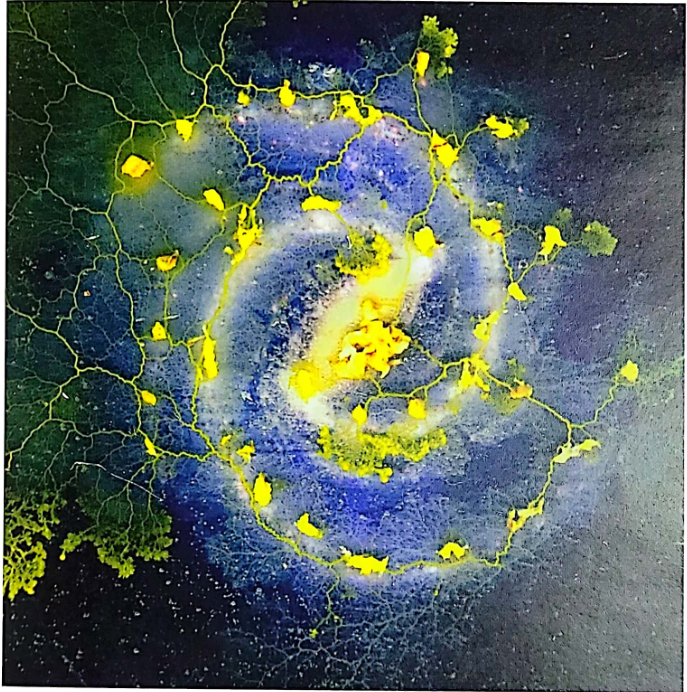
\includegraphics[width=0.25\textwidth]{./images/PhyrasumPolycephalum01.png}}
        \caption{Physarum propagating in an artist's impression of a galaxy. Image extracted from 'Atlas of Physarum Computing'. of A. Adamatzky \cite{Adamatzky2014}.}
        \label{fig:PhysarumPolycephalum01}    
    \end{figure} 
    \vskip 0.2cm
    %Parrafo 2
    As mentioned in the literature, myxomycetes are divided into two stages, the plasmodium and the fruiting bodies. Physarum Polycephalum 
        is a myxomycete that is in the plasmodial stage of its life cycle, in which the plasmodium is a bright yellow macroscopic multinucleate 
        coenocyte formed in a network of intertwined tubes. This stage of the life cycle is the one used for the study of this organism.\cite{Stephenson1994}
    \vskip 0.2cm
    %Parrafo 4
    Physarum Polycephalum is a very interesting organism for the study of biology and physics, since it has unique properties 
        that make it a very special organism. For example, Physarum Polycephalum is able to solve mazes, 
        find the shortest route between two points, and make complex decisions based on the 
        information it receives from its environment. In addition, the Physarum Polycephalum is able to learn and remember 
        information, and to adapt to its environment in a very efficient manner.
%%%%%%%%%%%%%%%%%%%%%%%%%%%%%%%%%%%%%%%%%%%%%%%%%%%%%%%%%%%%%%%%%%%%%%%%%%%%%%%%%%%%%%%%%%%%%%%%%%%%%%%%%%%%%%%%%%%%%%%%%%%%
\section{Algorithm}
\label{sec:algorithm}
    %Parrafo 1
    The proposed algorithm is based on the one described by Jeff Jones in his work 
        “From Pattern Formation to Material Computation: Multi-agent Modelling of Physarum Polycephalum” \cite{Jones2015}. 
    \vskip 0.2cm
    %Parrafo 2
    The algorithm is a cellular automaton that simulates the behavior of Physarum Polycephalum in a maze, so we need to define some concepts.
        First, let us denote $\mathbb{Z}$ as the set of integers, that is, $\mathbb{Z} = (-\infty, -1, 0, 1, \infty)$.
        and the length of any tuple $x$ as $|x|$. For all tuples $x$ and $y$ of the same length, let us denote $x \oplus y$
        as the tuple that results from the component-wise sum of $x$ and $y$, that is, $(x \oplus y)_i = x_i + y_i$ for all
        $i \in \mathbb{Z}$.
    \vskip 0.2cm
    %Parrafo 3
    Then we have that a cellular automaton is a tuple $(\mathbb{Z}^{n}, S, N, f)$ such that the n dimension is at least 1 where 
        $n \in \mathbb{Z}^{+}$, $S$ is a finite non-empty set of states, $N$ is a finite non-empty set of neighborhoods 
        belonging to $\mathbb{Z}^{n}$, and $f$ is a local transition function, that is, $f: S^N \rightarrow S$ where
        $S^N$ represents the set of all possible neighborhood configurations in $N$.
    \vskip 0.2cm
    %Parrafo 4
    Thus, the algorithm proposed in this work it is define as a cellular automaton $(\mathbb{Z}^{2}, S, N, f)$ where $n = 2$, 
        $S = \{0, 1, 2, 3, 4, 5, 6, 7, 8\}$, $N = \{0, 1, 2, 3, 4, 5, 6, 7, 8\}^9$, 
        and $f : \{0, 1, 2, 3, 4, 5, 6, 7, 8\}^9 \rightarrow \{0, 1, 2, 3, 4, 5, 6, 7, 8\}$,\( P = (C(x,y:t), N(x,y:t), M(x,y:t)) \) 
        represent the combined state, neighborhood, and memory of the cell at position \((x, y)\) at time \( t \). The transition function 
        \( f \) is defined as follows:
    \begin{equation*}
        \begin{aligned}
        f(P) = & \begin{cases}
            7 & \text{if } C(x,y:t) = 0 \\
              & \text{and } \exists N \in \{3, 4, 6\} \\
              & \text{and } M(x,y:t) = 0 \\
            6 & \text{if } C(x,y:t) = 1 \\
              & \text{and } \exists N \in \{5, 6\} \\
            2 & \text{if } C(x,y:t) = 2 \\
            3 & \text{if } C(x,y:t) = 3 \\
            5 & \text{if } C(x,y:t) = 4 \\
              & \text{and } \exists N \in \{3, 5, 6\} \\
              & \text{and } M(x,y:t) = 0 \\
              & \text{and } N \not\in \{0, 7\} \\
            0 & \text{if } C(x,y:t) = 5 \\
              & \text{and } M(x,y:t) \not\in \{5, 8\} \\
              & \text{and } N \not\in \{1, 3, 4, 6\} \\
            8 & \text{if } C(x,y:t) = 5 \\
              & \text{and the above condition is not met} \\
            4 & \text{if } C(x,y:t) = 7 \\
              & \text{and } \exists N \in \{3, 4, 6\} \\
            5 & \text{if } C(x,y:t) = 8 \\
            C(x,y:t) & \text{otherwise}
        \end{cases}
        \end{aligned}
    \end{equation*}
    %Table of states
    Where the states of the cellular automaton are defined as follows:
    \vskip 0.2cm
    \begin{table}[htbp]
        \caption{States of the cellular automaton}
        \begin{center}
        \begin{tabular}{|c|c|c|}
        \hline
        \textbf{Color}&\textbf{State}&\textbf{Description} \\
        \hline
        \cellcolor{blue} & 0 & Free Field  \\
        \cellcolor{royalblue} & 1 & Nutrient not found \\
        \cellcolor{red} & 2 & Repellent \\
        \cellcolor{black} & 3 & Initial point \\
        \cellcolor{yellow} & 4 & Contracting Gel \\
        \cellcolor{darkgreen} & 5 & Composite Gel \\
        \cellcolor{lemon} & 6 & Nutrient found \\
        \cellcolor{darkgray} & 7 & Physarum expansion \\
        \cellcolor{green} & 8 &  Uncompounded Gel\\
        \hline
        \end{tabular}
        \end{center}
    \end{table}
    \vskip 1cm
    %Parrafo x
    In the aforementioned source, the basic Physarum Polycephalum algorithm, originally designed to operate with a Von 
        Neumann neighborhood, is detailed. However, in the version proposed here, we chose to modify the neighborhood to a Moore neighborhood, 
        thus facilitating access to a larger number of neighbors for comparison and allowing us to obtain a clearer perspective on the optimal 
        direction for agent displacement.
    \section{Results}
    However, the use of the Moore neighborhood instead of the Von Neumann neighborhood introduces certain challenges not present in the original 
        algorithm. One of these challenges arises at corners (NW, NE, SW, SE), where the repeller could allow the agent to escape, contrary to 
        what is desired. To address this drawback, a solution was implemented that consists of placing an imaginary repeller in the corner when 
        two adjoining corners present repellents at a 90° angle to each other. This adjustment allows for the creation of a wider range of shapes, 
        as illustrated in Figs \ref{fig:physarumCircle1}, 
        \ref{fig:physarumRandom1} and \ref{fig:physarumObstacles1}. In this images the total number of cells is 50 x 50.
    \vskip 0.2cm
    \begin{figure}[htbp]
        \centerline{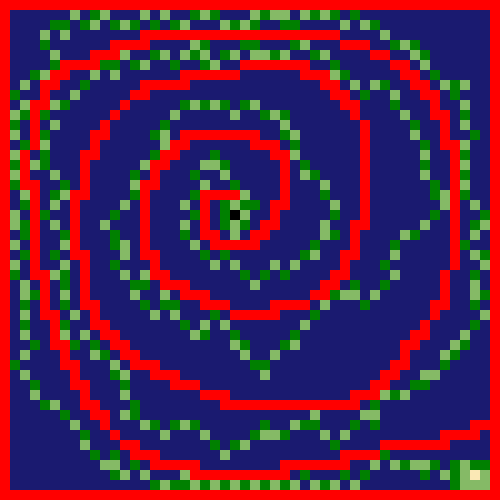
\includegraphics[width=0.25\textwidth]{./images/Circular1.png}}
        \caption{Physarum Polycephalum solving a spiral maze.} 
        \label{fig:physarumCircle1}    
    \end{figure}
    \begin{figure}[htbp]
        \centerline{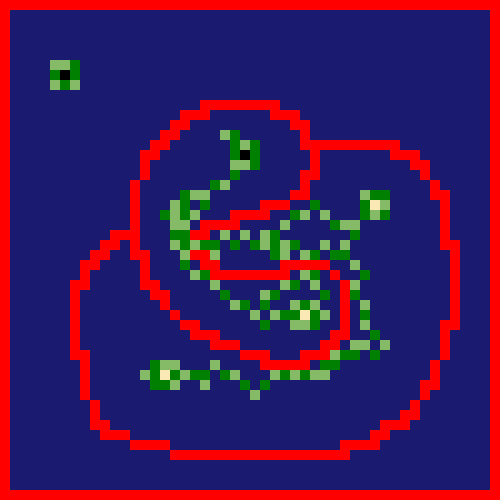
\includegraphics[width=0.25\textwidth]{./images/Random1.png}}
        \caption{Physarum Polycephalum solving a circular tipe maze.}
        \label{fig:physarumRandom1}    
    \end{figure}
    \begin{figure}[htbp]
        \centerline{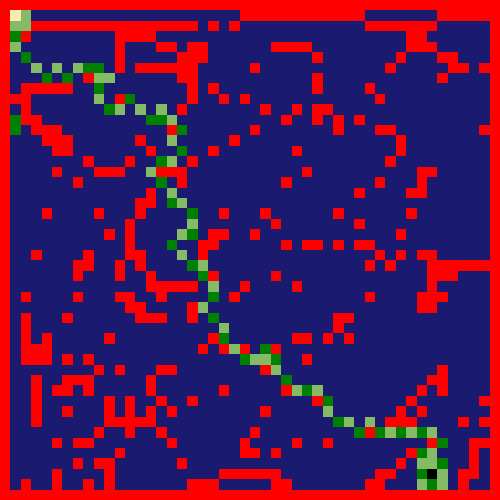
\includegraphics[width=0.25\textwidth]{./images/Obstaculos1.png}}
        \caption{Physarum Polycephalum solving a maze with obstacles.}
        \label{fig:physarumObstacles1}
    \end{figure}
    \vskip 0.5cm
    %Parrafo 3
    Thanks to the resolution of corner leakage by our algorithm, it is possible to generate more 
        diverse mappings of caves and catacombs. This approach significantly improves our understanding 
        of the topography of the explored area. In addition, the diversity in mapping facilitates the identification 
        of the number and variety of available paths, which has been implemented by an image mapping algorithm that 
        assists in the graphical representation of such topography, as shown in Fig \ref{fig:CaveSystemPhysarum}. The space 
        explored by the algorithm is 1000 x 1000 cells and have a total of 146135 red cells or repellent cells.
    \vskip 0.2cm
    \begin{figure}[htbp]
        \centerline{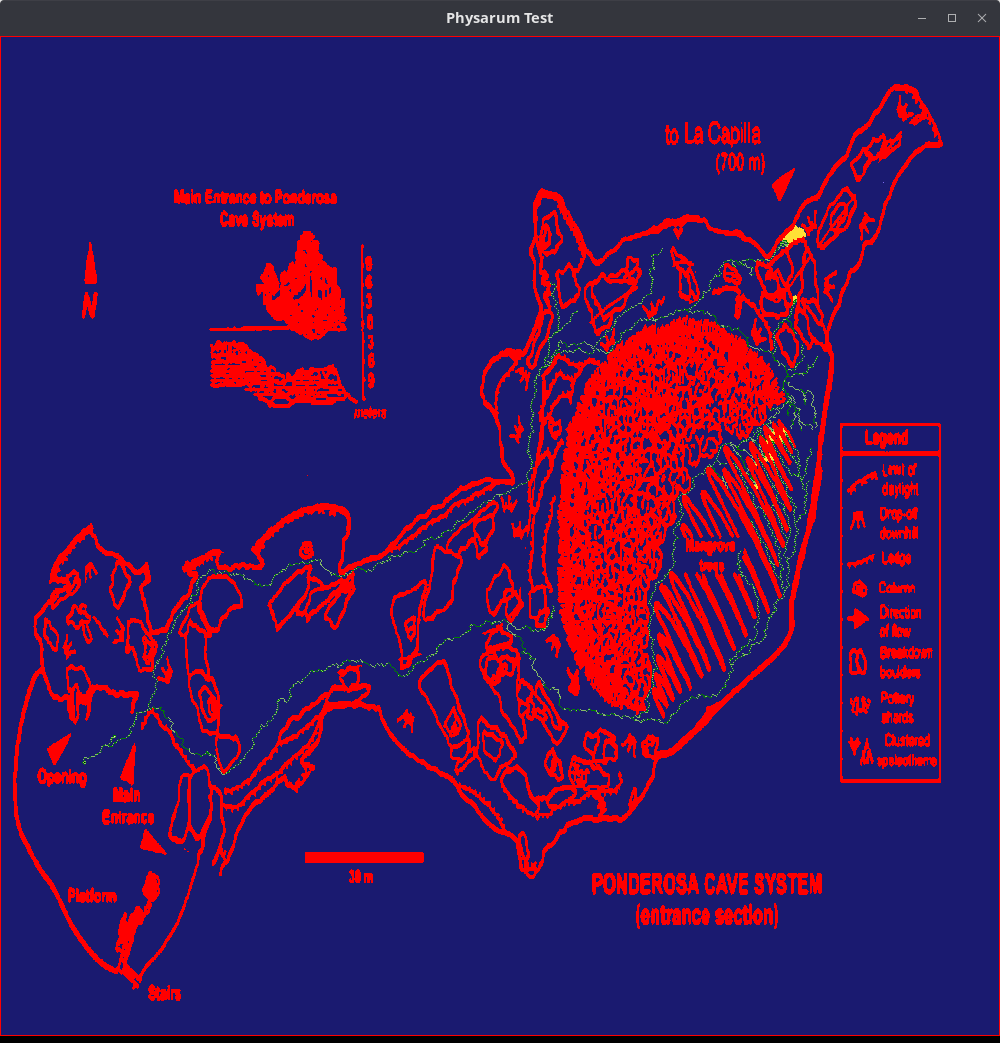
\includegraphics[width=0.40\textwidth]{./images/CaveSystemPhysarum.png}}
        \caption{Cave system mapping using Physarum Polycephalum.}
        \label{fig:CaveSystemPhysarum}
    \end{figure}
    \vskip 0.2cm
    Also the algorithm has been tested in a real environment, where it has been able to generate 
        optimal routes in the Paris Catacomb, as shown in Fig \ref{fig:Catacomb}. The space
        explored by the algorithm is 1000 x 1000 cells.
    \vskip 0.2cm
    \begin{figure}[htbp]
        \centerline{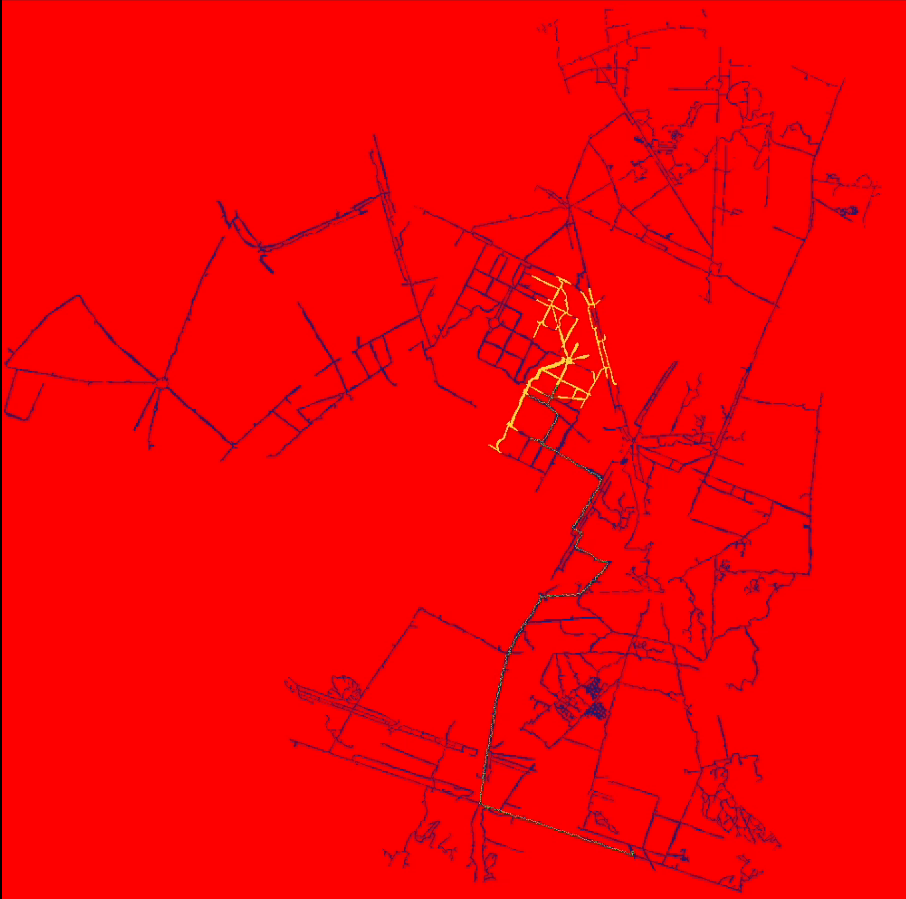
\includegraphics[width=0.40\textwidth]{./images/CatacoumbParis.png}}
        \caption{Catacomb mapping using Physarum Polycephalum, uses 5264 steps to get route.}
        \label{fig:Catacomb}
    \end{figure}
    %Parrafo 4
    It should be noted that since the algorithm is bio-inspired, the function that simulates plasmodium behavior 
        is assigned in a pseudo-random manner to an adjacent neighbor, with a probability of 1/8. This feature allows 
        the expansion of the algorithm to take a circular form rather than a square or linear expansion. However, by 
        modifying the likelihood function, it is possible to achieve a more irregular rather than merely circular expansion.
\section{Conclusions}
\label{sec:conclusions}
    %Parrafo 1
    In this work, we have presented a routing algorithm based on Physarum Polycephalum for navigation in caves and catacombs. 
        The algorithm is implemented in real time and is designed to map complex subterranean environments. The algorithm takes 
        advantage of the adaptive and explorative properties of the mold to determine optimal routes through natural mazes and 
        subterranean structures. It stands out for its ability to adapt instantly to changes and its efficiency in continuous exploration 
        without manual intervention. Experimental results indicate that the algorithm not only improves the efficiency of path generation, 
        but also demonstrates robustness to obstacles and topographic variations. These characteristics offer new tools for archaeological 
        and geological exploration, advancing significantly towards the automation of subway exploration.
    \vskip 0.2cm
    %Parrafo 2
    Future work will focus on the development of a more efficient algorithm that can generate optimal routes in real time, 
        as well as on the implementation of a more sophisticated image mapping algorithm that can assist in the graphical 
        representation of the topography of the explored area. In addition, we will explore the possibility of using the algorithm 
        in other types of environments, such as forests, deserts, and mountains, to determine its effectiveness in generating optimal 
        routes in these environments.
    \vskip 0.2cm
    %Parrafo 3
    In conclusion, the algorithm proposed in this work is a promising tool for the exploration of caves and catacombs, 
        as well as for the automation of subway exploration. The algorithm is efficient, robust, and adaptable, and has the 
        potential to revolutionize the way we explore and map subterranean environments. We believe that the algorithm will 
        have a significant impact on the fields of archaeology, geology, and exploration, and we look forward to further 
        developing and refining the algorithm in the future.
%%%%%%%%%%%%%%%%%%%%%%%%%%%%%%%%%%%%%%%%%%%%%%%%%%%%%%%%%%%%%%%%%%%%%%%%%%%%%%%%%%%%%%%%%%%%%%%%%%%%%%%%%%%%%%%%%%%%%%%%%%%%

\bibliographystyle{ieeetr}
\bibliography{reference.bib}

\end{document}
